\documentclass[
size=17pt,
paper=smartboard,
mode=present,
display=slidesnotes,
style=paintings,
nopagebreaks,
blackslide,
fleqn]{powerdot}

% styles: sailor, paintings
% wj capsules prettybox
% mode = handout or present


\usepackage{amsmath,graphicx,color,amsfonts}
\usepackage[brazilian]{babel}
\usepackage[utf8]{inputenc}
\newcommand{\palette}{Moitessier}


% palettes:
%    - sailor: Sea, River, Wine, Chocolate, Cocktail 
%    - paintings: Syndics, Skater, GoldenGate, Moitessier, PearlEarring, Lamentation, HolyWood, Europa, MayThird, Charon 

\newcommand{\cursopequeno}{EC01039 CG\underline{PI}}
\newcommand{\cursogrande}{\Large EC01039 -- Computação gráfica e \underline{processamento de imagem}}



\author{Ronaldo de Freitas Zampolo\\FCT-ITEC-UFPA}
\date{2020.2}


\pdsetup{
	lf = {\cursopequeno},
	rf = {Introdução ao PDI}, 
	cf = {\arabic{slide}~/~\pageref*{lastslide}},
	palette = {\palette}, 
	randomdots={false}
}

%opening
\title{\cursogrande\\ \vspace{1cm}Introdução ao processamento digital de imagem}
\author{Ronaldo de Freitas Zampolo\\FCT-ITEC-UFPA}
\date{ }

\begin{document}
   \maketitle[randomdots={false}]
   \begin{slide}{Agenda}
      \tableofcontents[content=sections]
   \end{slide}

   \section[ slide = true]{Motivação}
      \begin{slide}[toc=]{Principais interesses}
		\begin{itemize}
		      \item Melhoramento da informação visual (interpretação humana)
		      \item Adequação dos dados para armazenamento
		      \item Adaptação para transmissão
		      \item Representação para visão computacional (interpretação pela máquina)
		\end{itemize}
      \end{slide}


   \section[ slide = true]{O que é processamento digital de imagens?}
      \begin{slide}[toc=]{Processamento digital de imagens: o que é?}
         \begin{itemize}
            \item Imagem: função bidimensional $f:\mathbb{R}^2\rightarrow \mathbb{R}$ 
            \item Coordenadas espaciais: $(x,y)$
            \item Intensidade: $f(x,y)$
            \item Imagem \underline{digital}: $x$, $y$, e $f(x,y)$ são discretos
            \item Elemento de uma imagem: \emph{pixel} ou \emph{pel} (picture element)
            \item Limites do processamento de imagens e outras áreas relacionadas: visão computacional, e análise de imagem
            \item Paradigma dos processos de três níveis:
            \begin{description}
               \item [Nível baixo:]Operações primitivas; entrada: imagens; saída: imagens; ex.: redução de ruído, modificação de contraste, aguçamento, restauração, etc.
               \item [Nível médio:]Entrada: imagem; saída: atributos; ex.: segmentação, classificação, etc.
               \item [Nível alto:] ``Dar sentido'', realizar funções congnitivas associadas à visão. 
            \end{description}
         \end{itemize}
      \end{slide}

   \section[ slide = true]{As origens do processamento digital de imagens}
      \begin{slide}[toc=]{Transmissão de imagens}
         \begin{itemize}
            \item Primeiras aplicações: indústria de jornais
            \item Transmissão de Londres para Nova York (1921): de uma semana para 3 horas
	    \footnote{\tiny{Sistemas Bartlane: \url{http://en.wikipedia.org/wiki/Bartlane_cable_picture_transmissionl_system}}}\\
            \begin{center}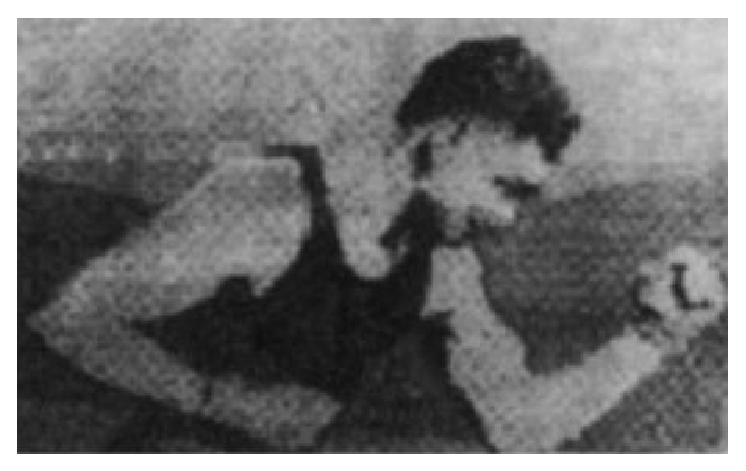
\includegraphics[width=0.6\textwidth]{figs/bartlane_1921}\end{center}
         \end{itemize}         
      \end{slide}

      \begin{slide}[toc=]{Melhoramentos}
         \begin{itemize}
            \item Aumento no número de níveis de cinza (de 5 para 15, 1929)
            \begin{center}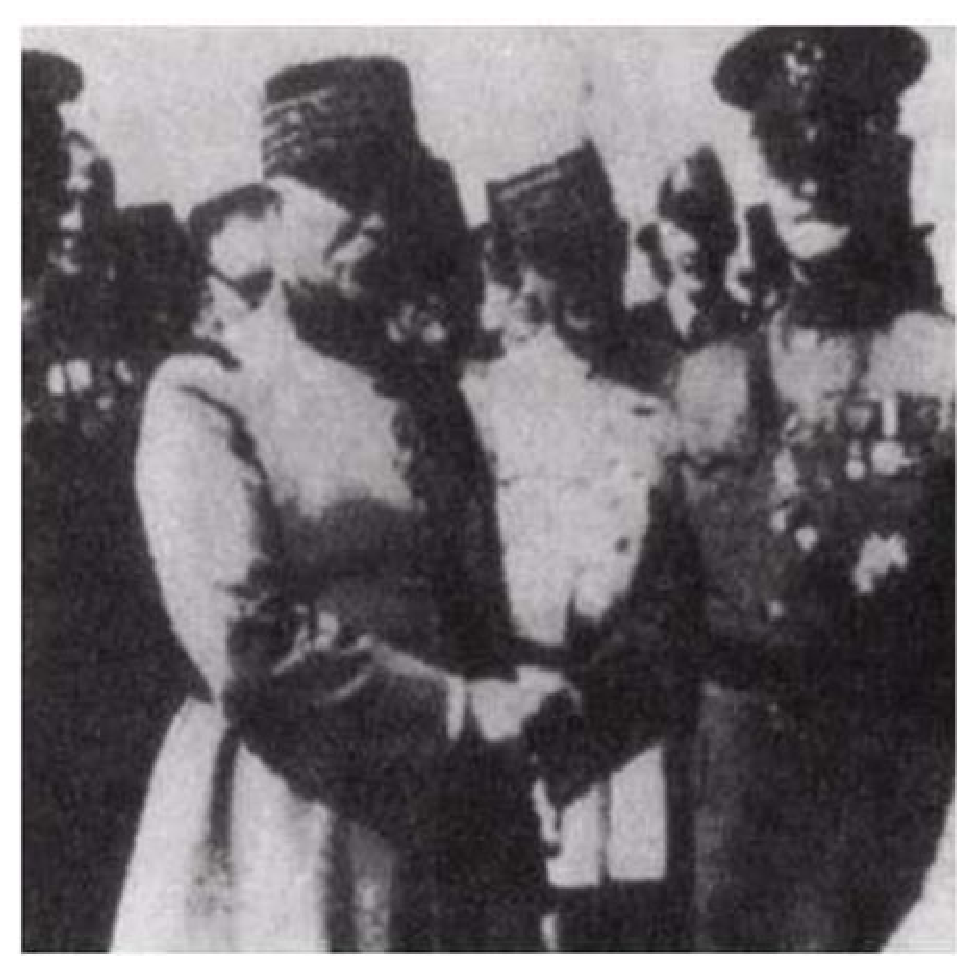
\includegraphics[width=0.5\textwidth]{figs/pershing_foch_1929}\end{center}
         \end{itemize}         
      \end{slide}

      \begin{slide}[toc=]{Mas... antes do surgimento dos computadores?}
	      \begin{itemize}
		      \item Não era ainda processamento \emph{digital}: não existiam computadores 
		      \item Mesmo depois de haverem computadores:
			      \begin{itemize}[type=1]
				      \item Volume de dados em imagens é muito grande
				      \item Foi necessário esperar avanços nos sistemas de armazenamento e transmissão
			      \end{itemize}
	      \end{itemize}
      \end{slide}
      
      \begin{slide}[toc=]{Programa espacial e melhores computadores}
         \begin{itemize}
            \item Fotografias da superfície lunar (Ranger 7, 1964)
            \begin{center}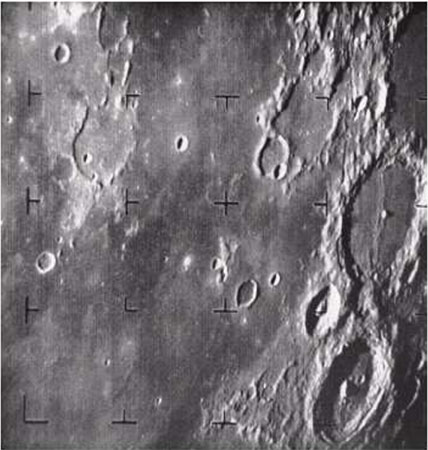
\includegraphics[width=0.45\textwidth]{figs/ranger7_1964}\end{center}
         \end{itemize}         
      \end{slide}
      
      
   \section[ slide = true]{Áreas de aplicação}
   \begin{slide}[toc=]{Imagens fomadas por raios gama}
      \begin{itemize}
         \item Astronomia, medicina, manutenção ...
         \begin{center}
		 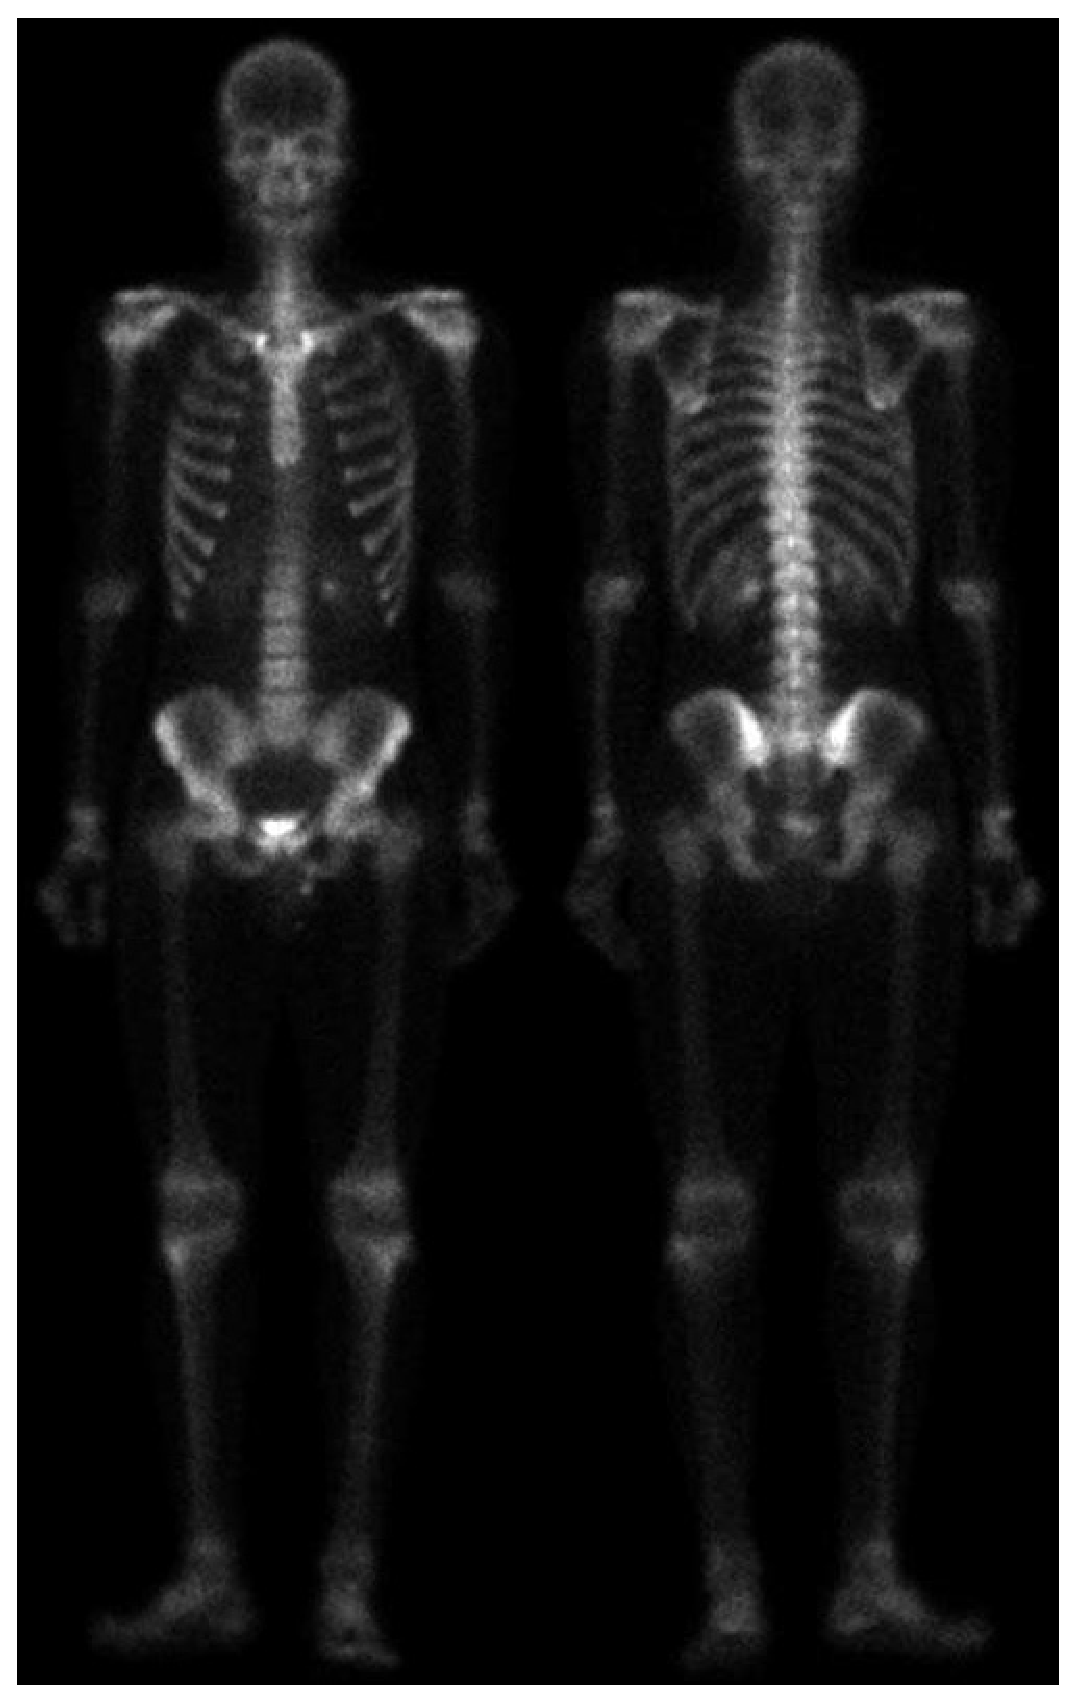
\includegraphics[width=0.18\textwidth]{figs/Fig0106a}
		 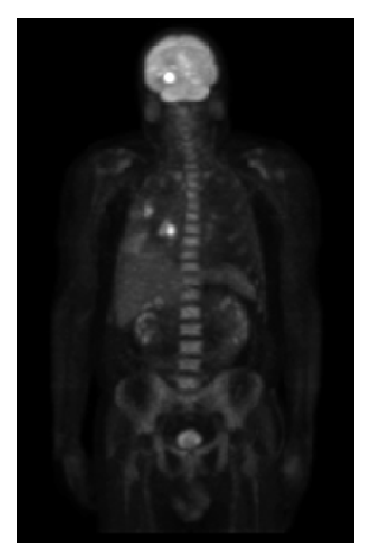
\includegraphics[width=0.18\textwidth]{figs/Fig0106b}\\
		 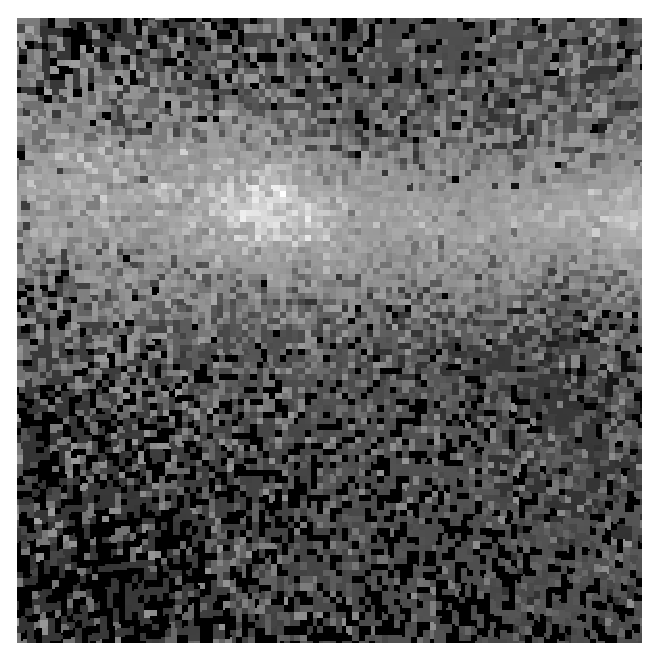
\includegraphics[width=0.18\textwidth]{figs/Fig0106c}
		 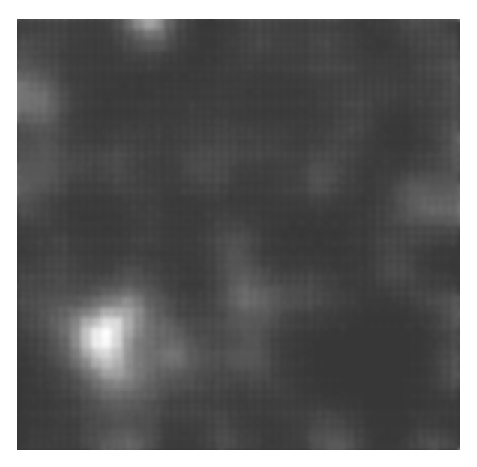
\includegraphics[width=0.18\textwidth]{figs/Fig0106d}\\
         \tiny{(a: escaneamento ósseo; b: PET; c: Cygnus loop; d: válvula de reator nuclear)}
         \end{center}
      \end{itemize}
   \end{slide}
   
   \begin{slide}[toc=]{Imagens fomadas por raios X}
      \begin{itemize}
         \item Astronomia, medicina, manutenção ...
         \begin{center}
         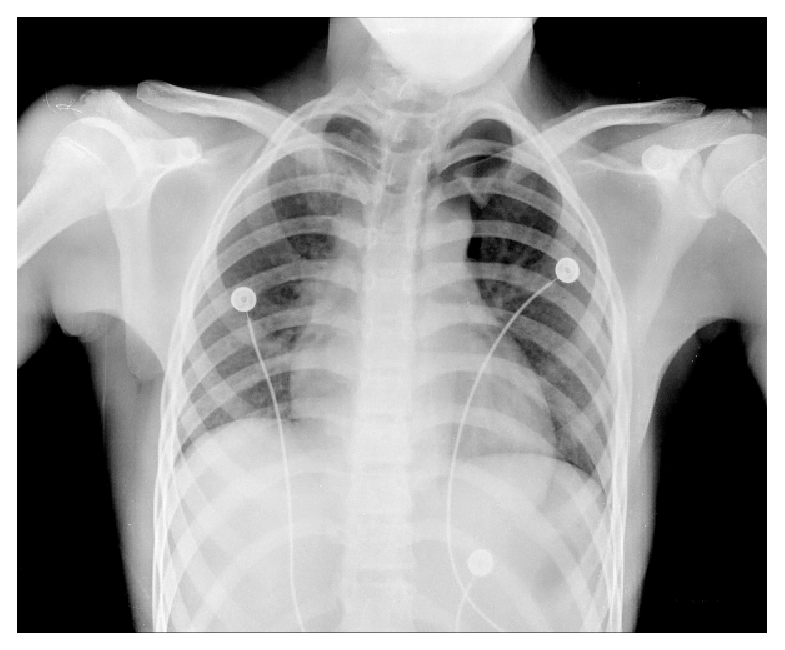
\includegraphics[width=0.2\textwidth]{figs/Fig0107a}
         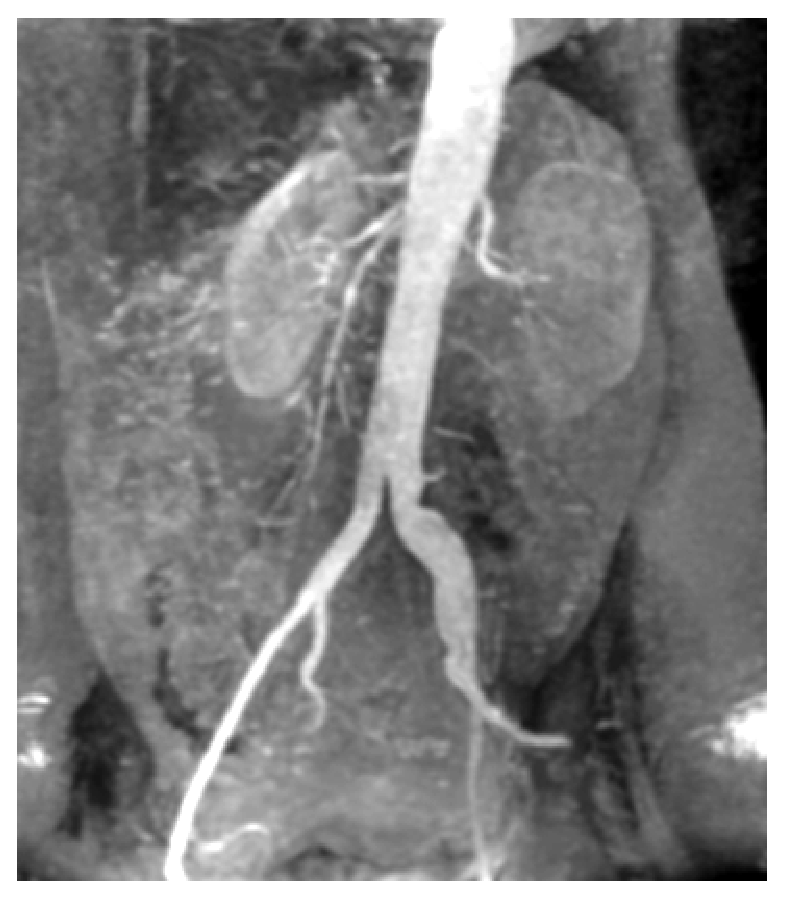
\includegraphics[width=0.2\textwidth]{figs/Fig0107b}\\
         %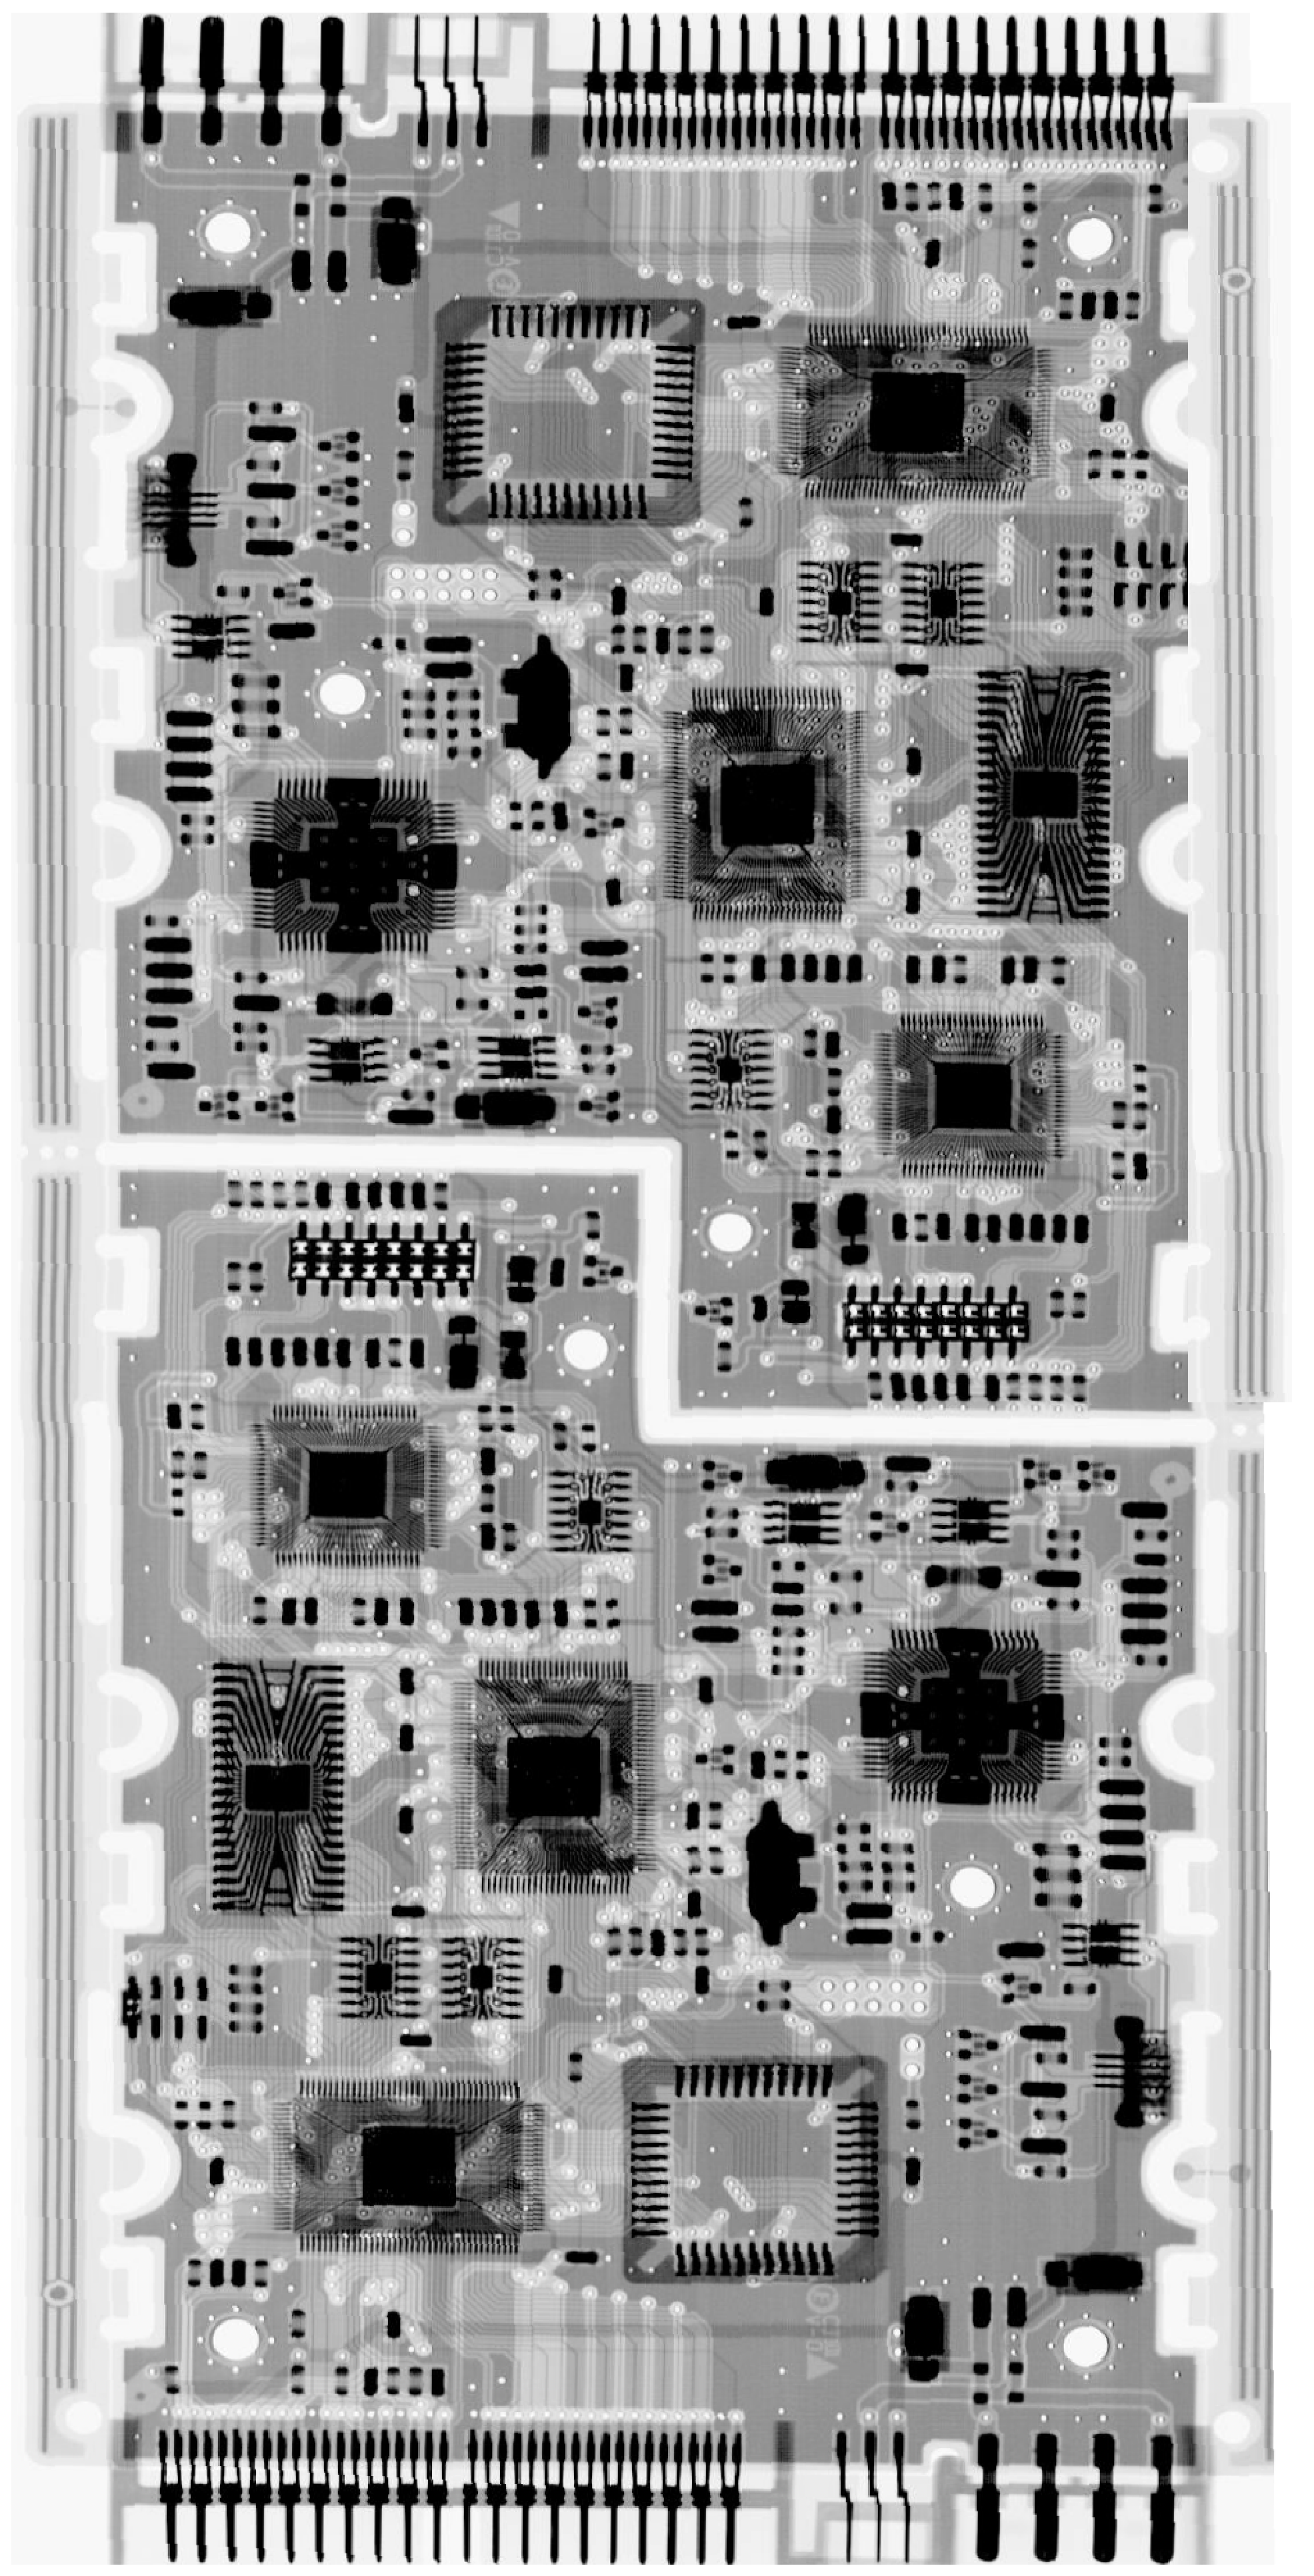
\includegraphics[width=0.24\textwidth]{figs/Fig0107d}\\
         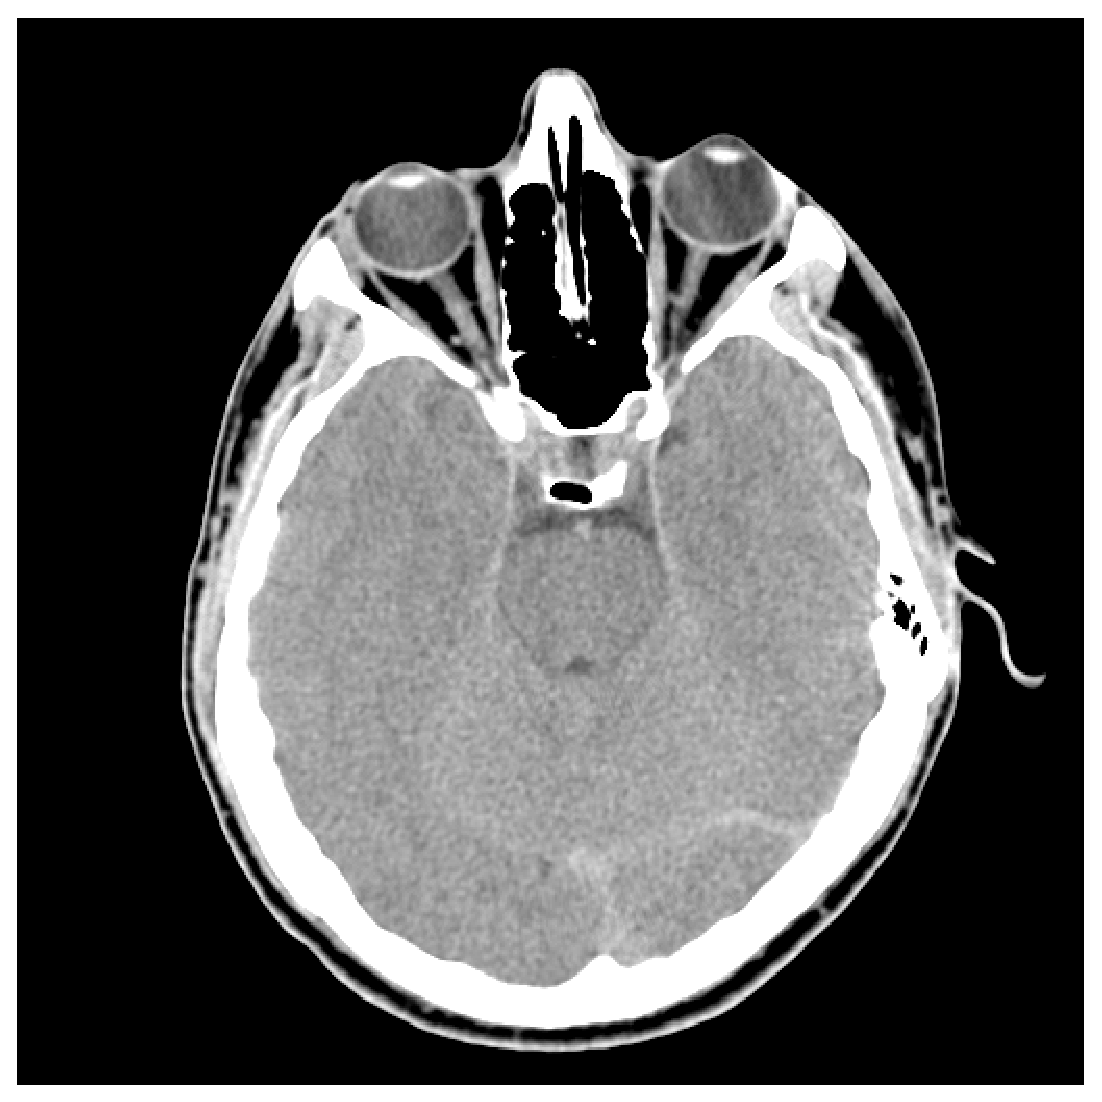
\includegraphics[width=0.2\textwidth]{figs/Fig0107c}
         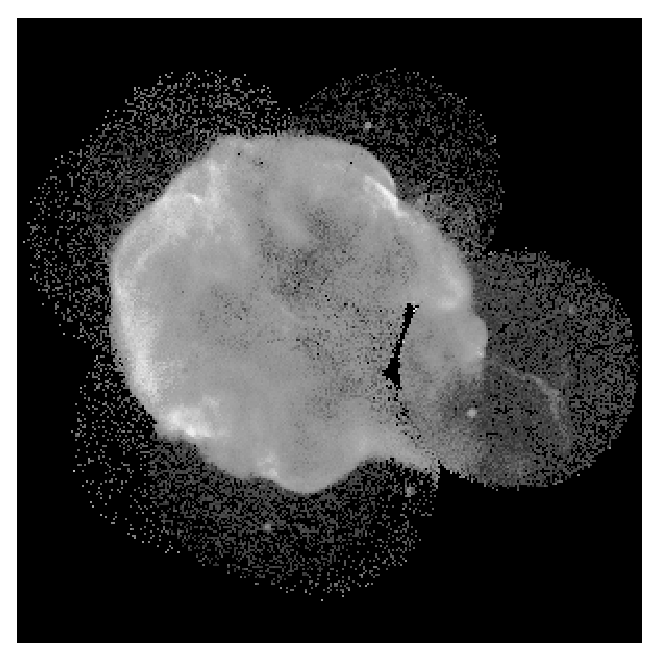
\includegraphics[width=0.2\textwidth]{figs/Fig0107e}\\
         \tiny{(a: rx torax; b: angiograma de aorta; c: TC de cabeça; d: Cygnus loop)}
         \end{center}
      \end{itemize}
   \end{slide}

   \begin{slide}[toc=]{Outras modalidades}
      \begin{itemize}
         \item Imagens na banda ultravioleta
         \item Imagens na banda visível
         \item Imagens na banda infravermelha
         \item Imagens da faixa de micro ondas
         \item Imagens na faixa de rádio
         \item Imagens ultra sônicas
         \item Imagens sísmicas
         \item Imagens de sonar
      \end{itemize}
   \end{slide}


   \section[ slide = true]{Passos fundamentais em PDI}
   \begin{slide}[toc=]{Passos fundamentais}
      
       \begin{center}
         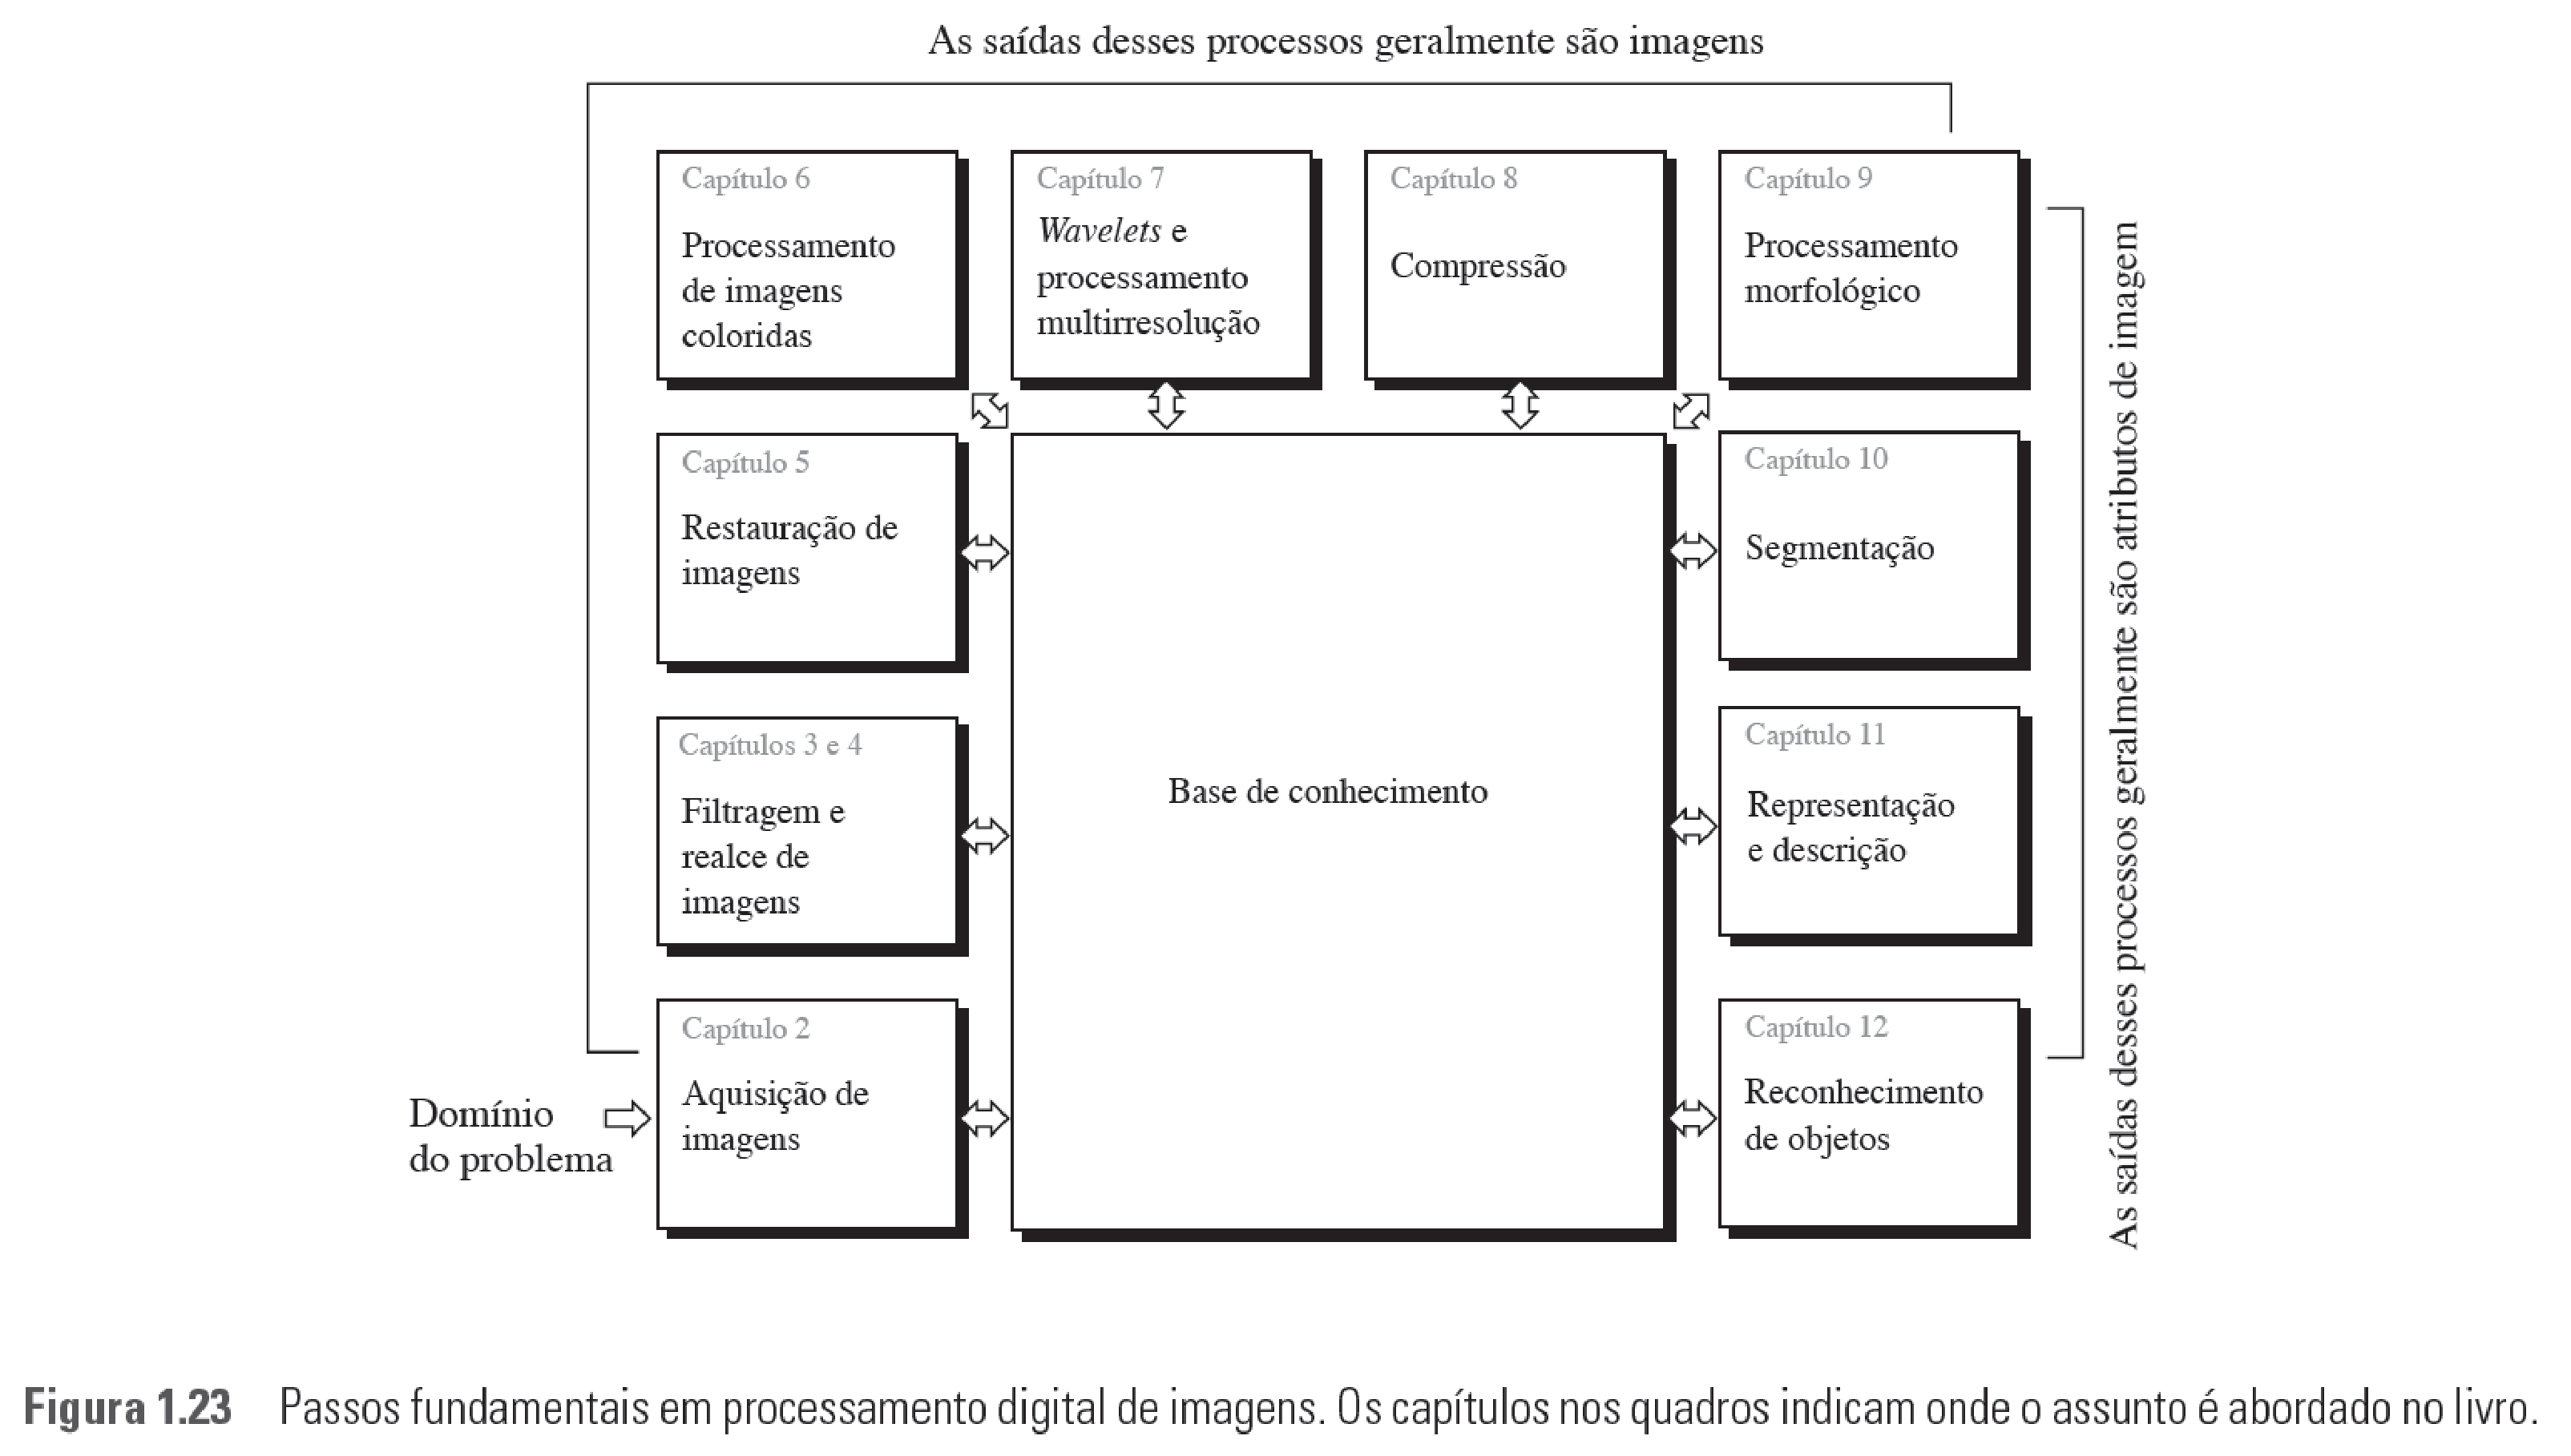
\includegraphics[width=1\textwidth]{figs/Fig0123}
         \end{center}
      
   \end{slide}
   
   \section[ slide = true]{Componentes de um sistema de PDI}
      \begin{slide}[toc=]{Componentes}
         \begin{center}
         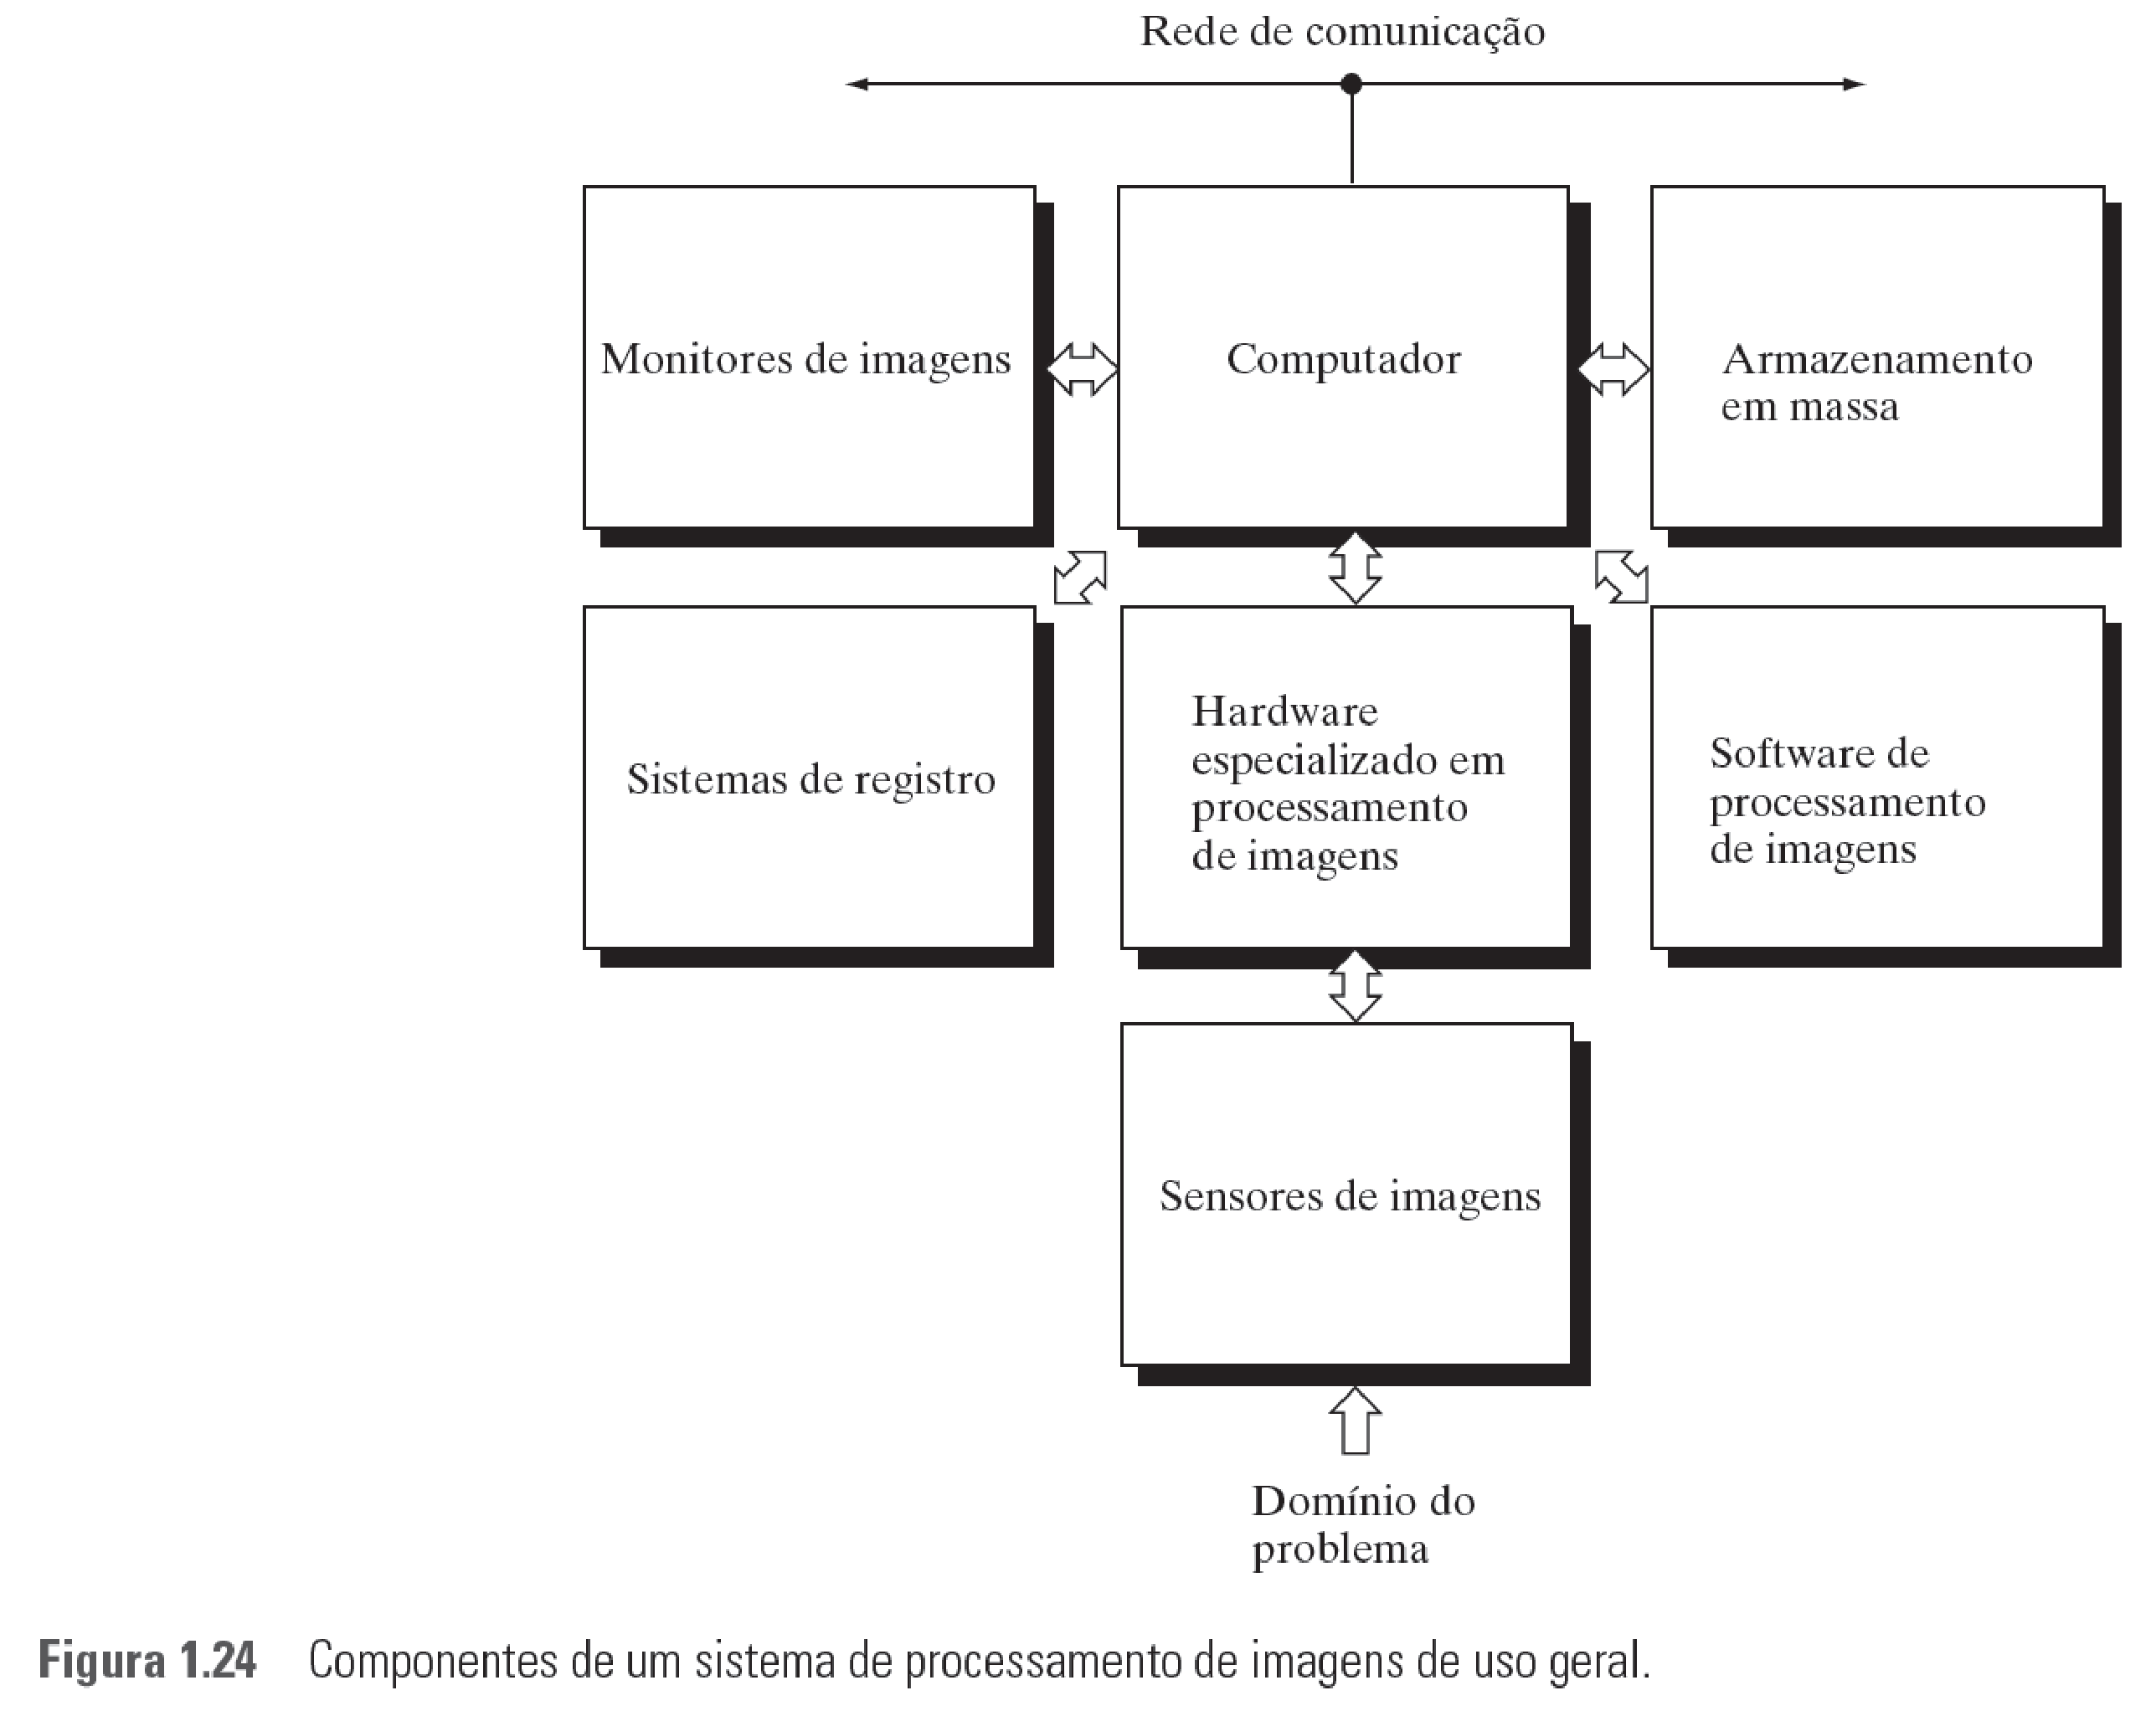
\includegraphics[width=.7\textwidth]{figs/Fig0124}
         \end{center}
      \end{slide}
      
\end{document}
